\documentclass[aspectratio=169]{beamer}
\usepackage{will_handley_beamer}
\usepackage{title_page}
\usepackage{slashed}

% Commands
% --------
% - \arxiv{arxiv number}
% - \cols{width}{lh column}{rh column}
% -  \begin{fig(left|right)}[fractional width (e.g 0.6) ]{name of image}
%        content of other column
%    \end{fig(left|right)}

% Talk details
% ------------
\title{Next-generation astrophysical inference}
\subtitle{across the interdisciplinary frontier}
\date{29\textsuperscript{th} April 2024}

\begin{document}

\begin{frame}
    \titlepage
\end{frame}

\begin{frame}
    \frametitle{Beginning the golden age of astronomy data}
    \begin{columns}
        \column{0.45\textwidth}
        \begin{itemize}
            \item Over our research lifetimes we will see next-generation data rates across the electromagnetic spectrum \& beyond:
                \begin{description}
                    \item[Radio] SKA \textit{et al}
                    \item[Micro] SO/CMB-S4
                    \item[IR] JWST, Roman (WFIRST)
                    \item[Optical] Euclid, DESI, Rubin (LSST), EELT
                    \item[X-ray] Athena
                    \item[Gamma-ray] e-ASTROGAM
                    \item[Gravitational] LIGO/Virgo/Kagra + LISA
                    \item[Particle] CTA, IceCube, KM3NeT
                \end{description}
        \end{itemize}
        \column{0.55\textwidth}

        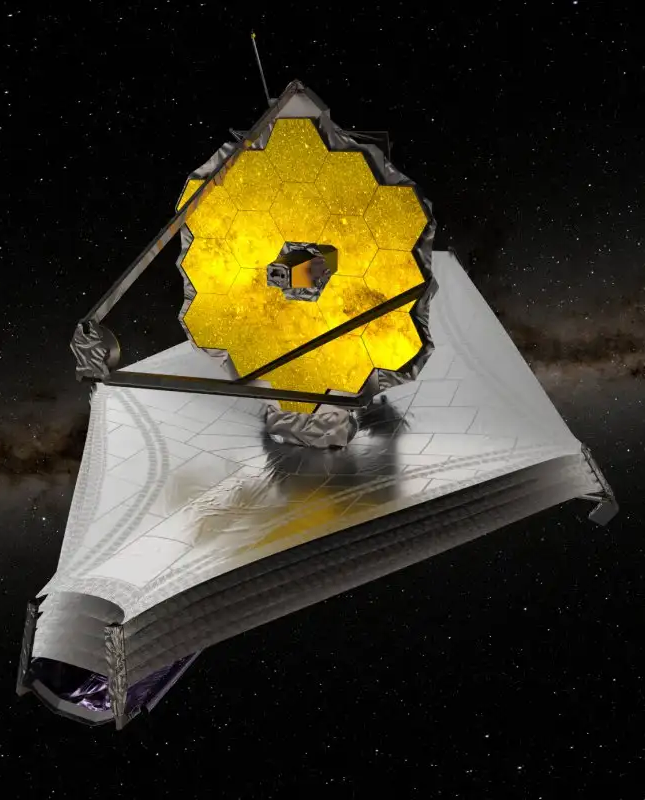
\includegraphics[height=0.145\textwidth]{figures/telescopes/jwst}%
        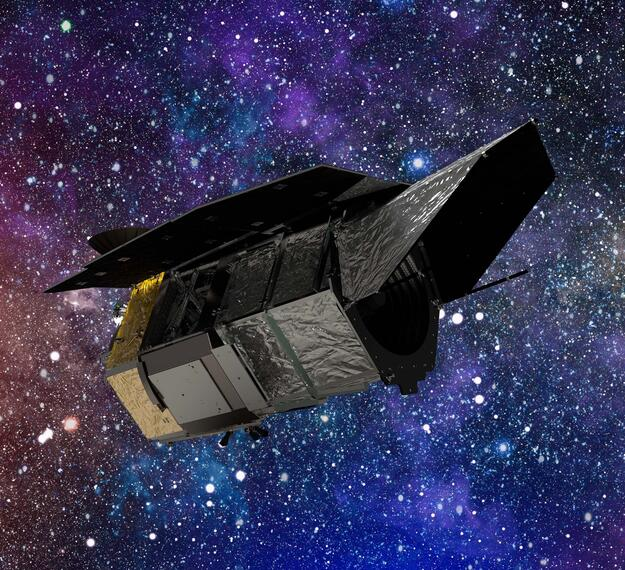
\includegraphics[height=0.145\textwidth]{figures/telescopes/roman}%
        \includegraphics[height=0.145\textwidth]{figures/telescopes/euclid}%
        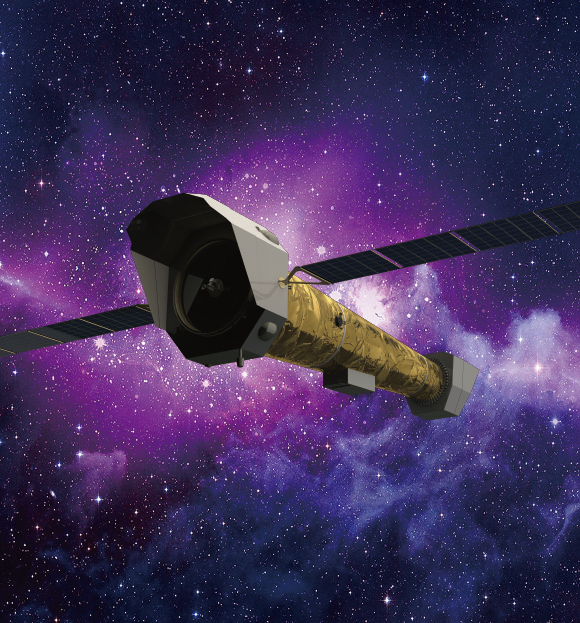
\includegraphics[height=0.145\textwidth]{figures/telescopes/athena}%
        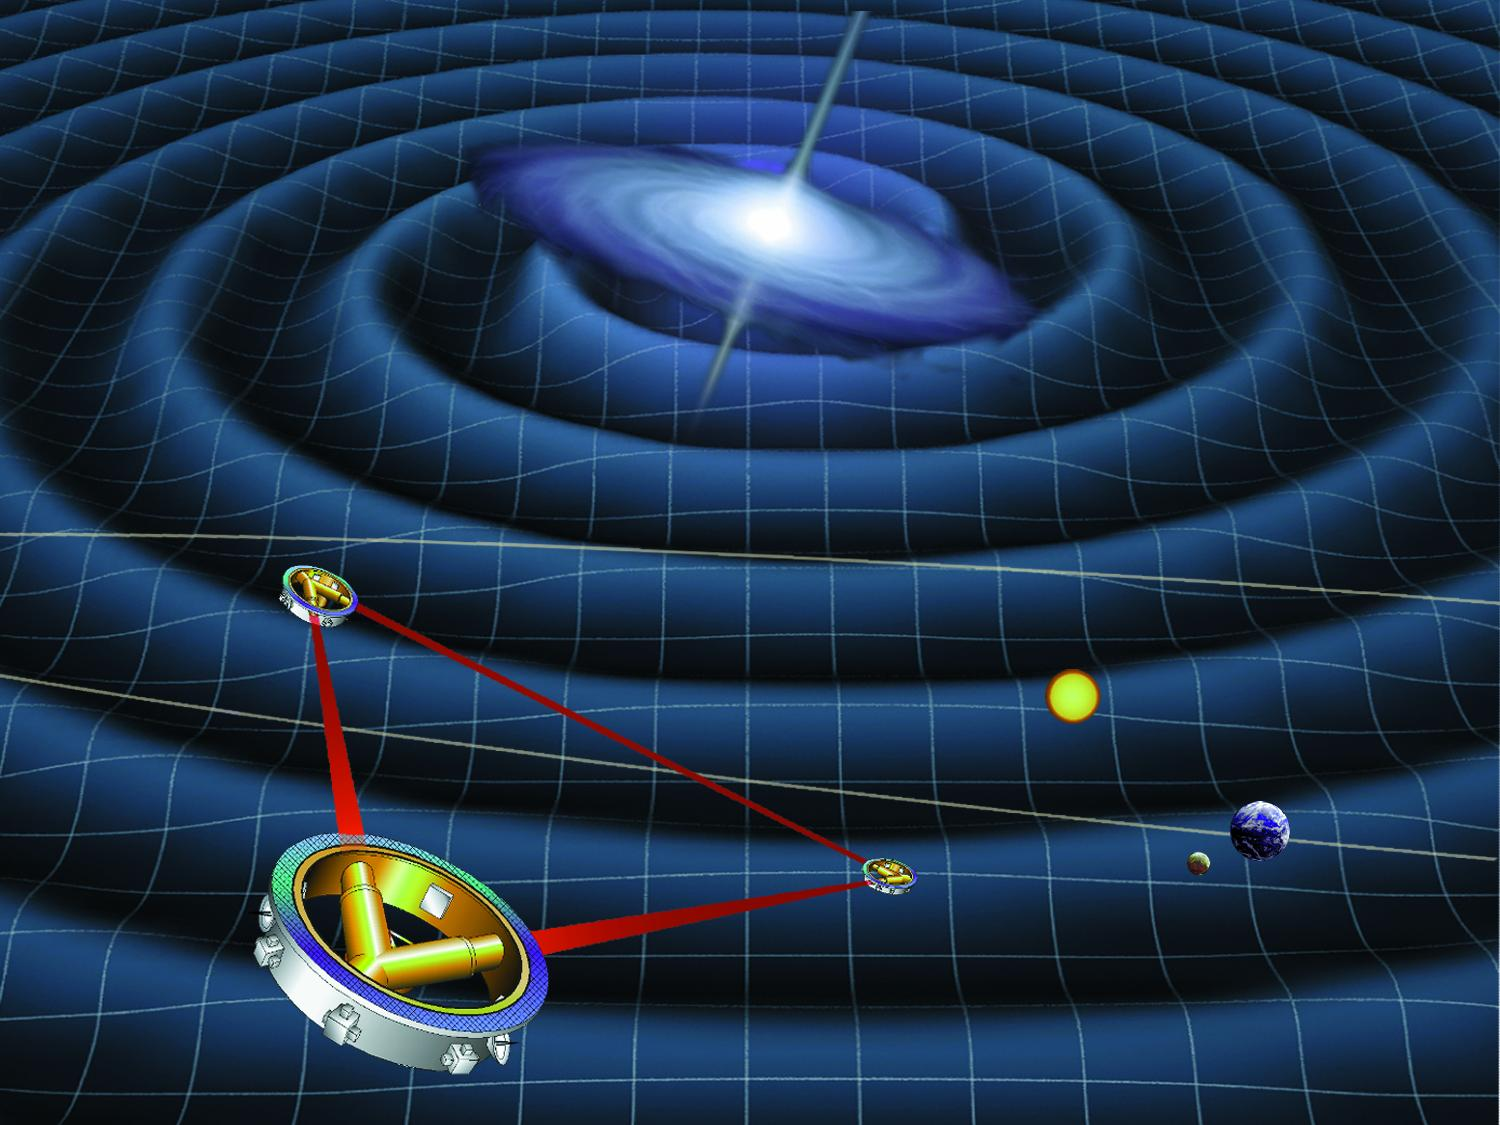
\includegraphics[height=0.145\textwidth]{figures/telescopes/lisa}%
        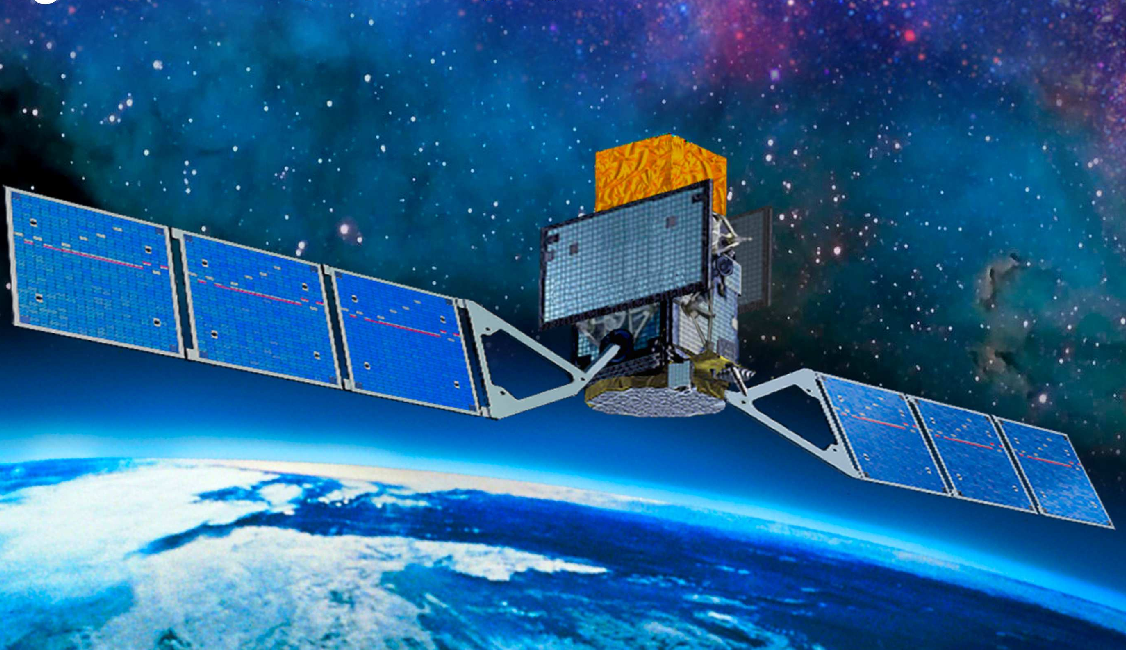
\includegraphics[height=0.145\textwidth]{figures/telescopes/e-ASTROGAM}%
        \vspace{-1pt}

        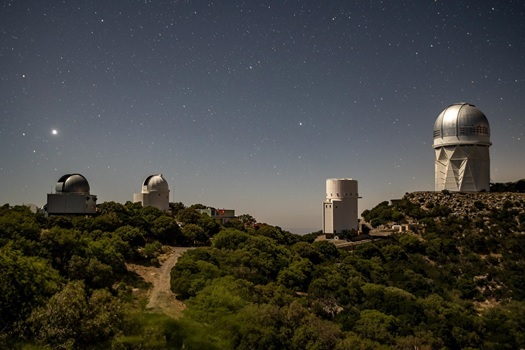
\includegraphics[height=0.15183\textwidth]{figures/telescopes/desi}%
        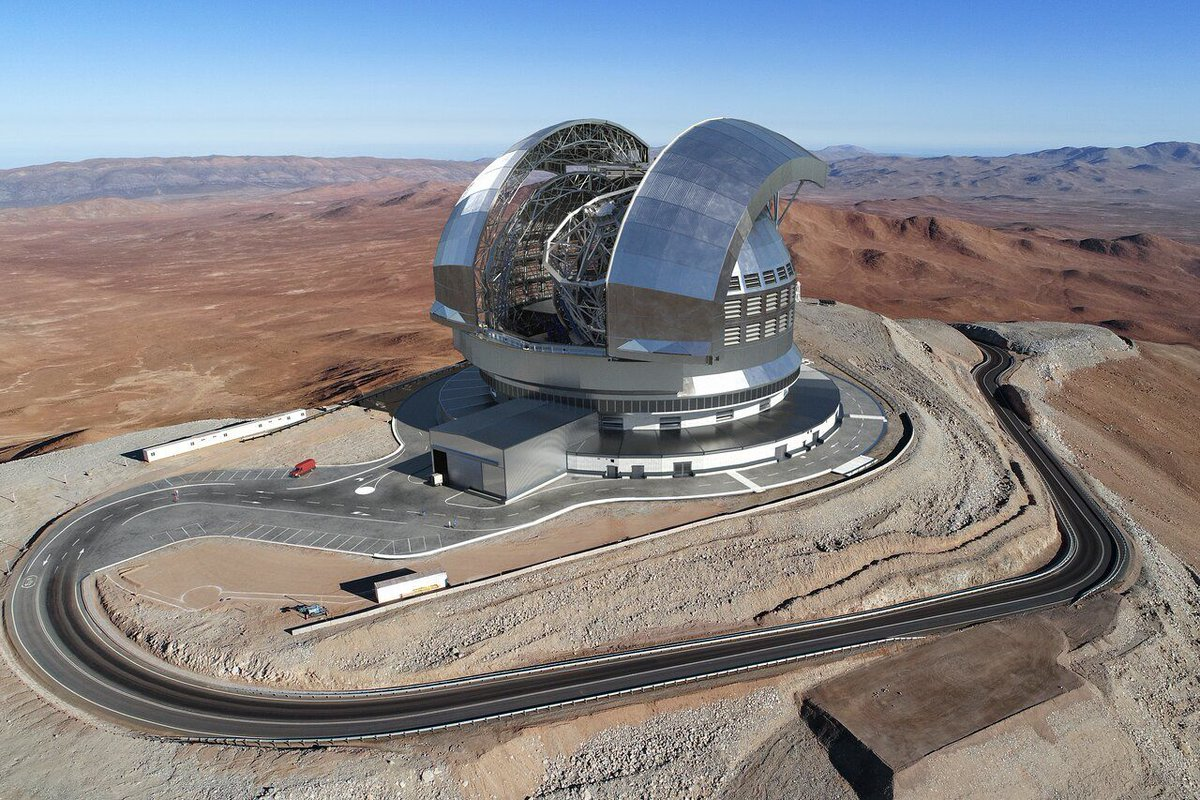
\includegraphics[height=0.15183\textwidth]{figures/telescopes/eelt}%
        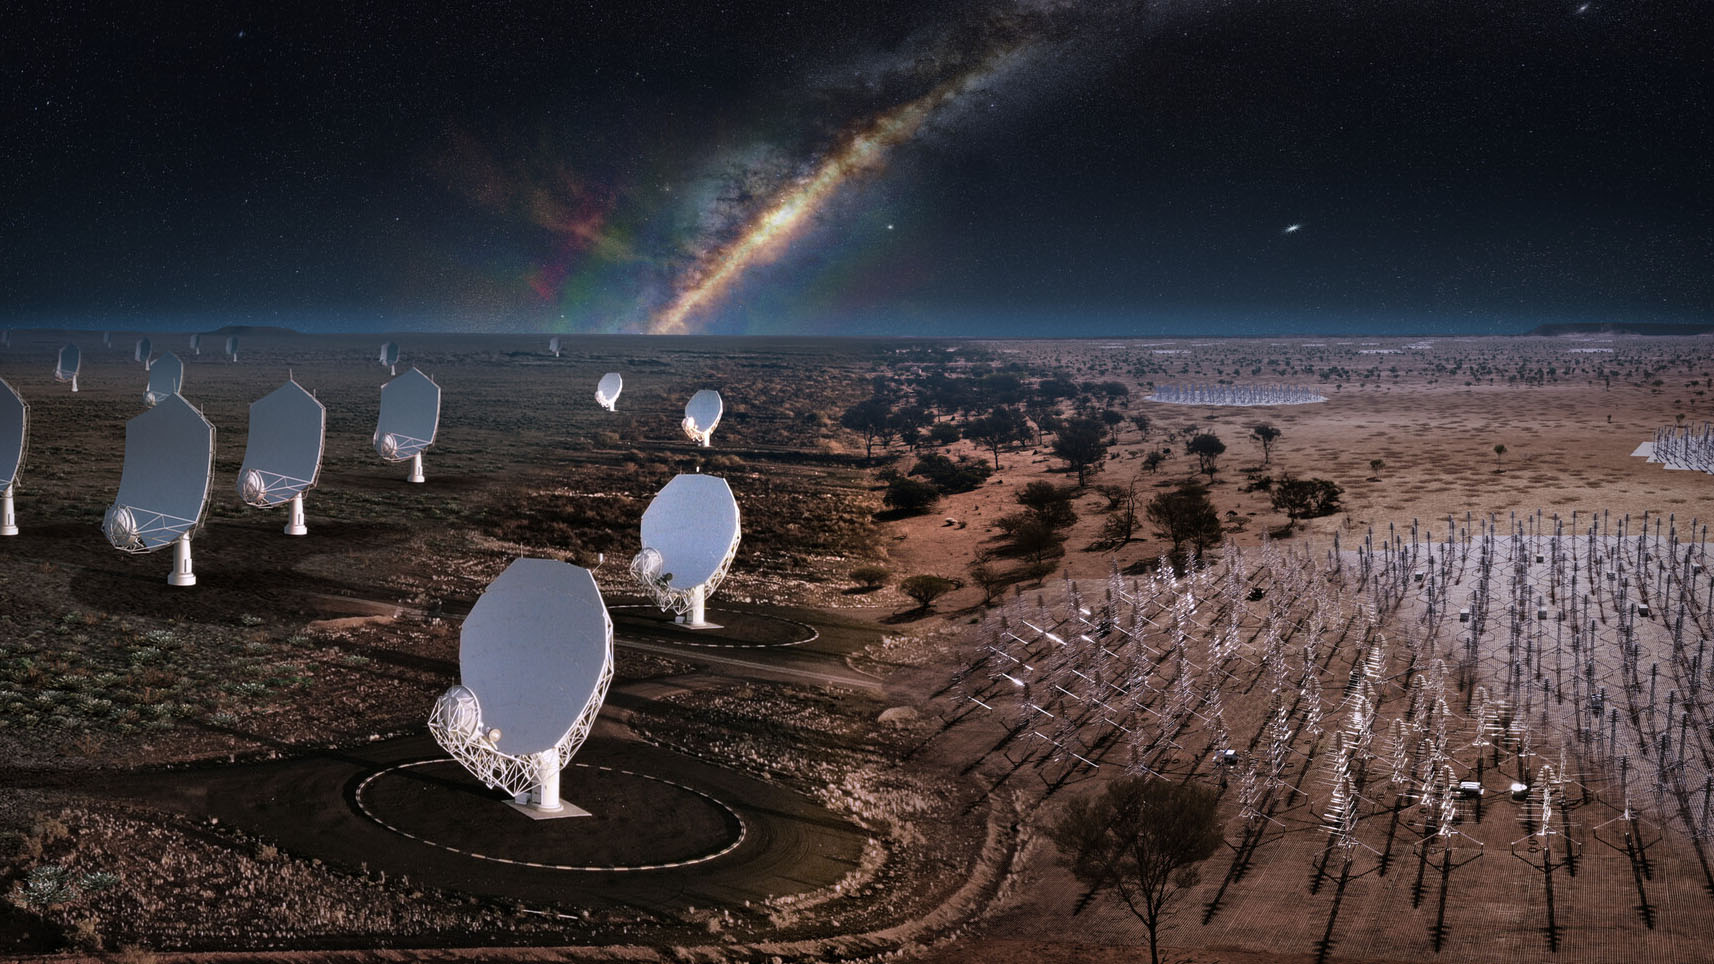
\includegraphics[height=0.15183\textwidth]{figures/telescopes/ska}%
        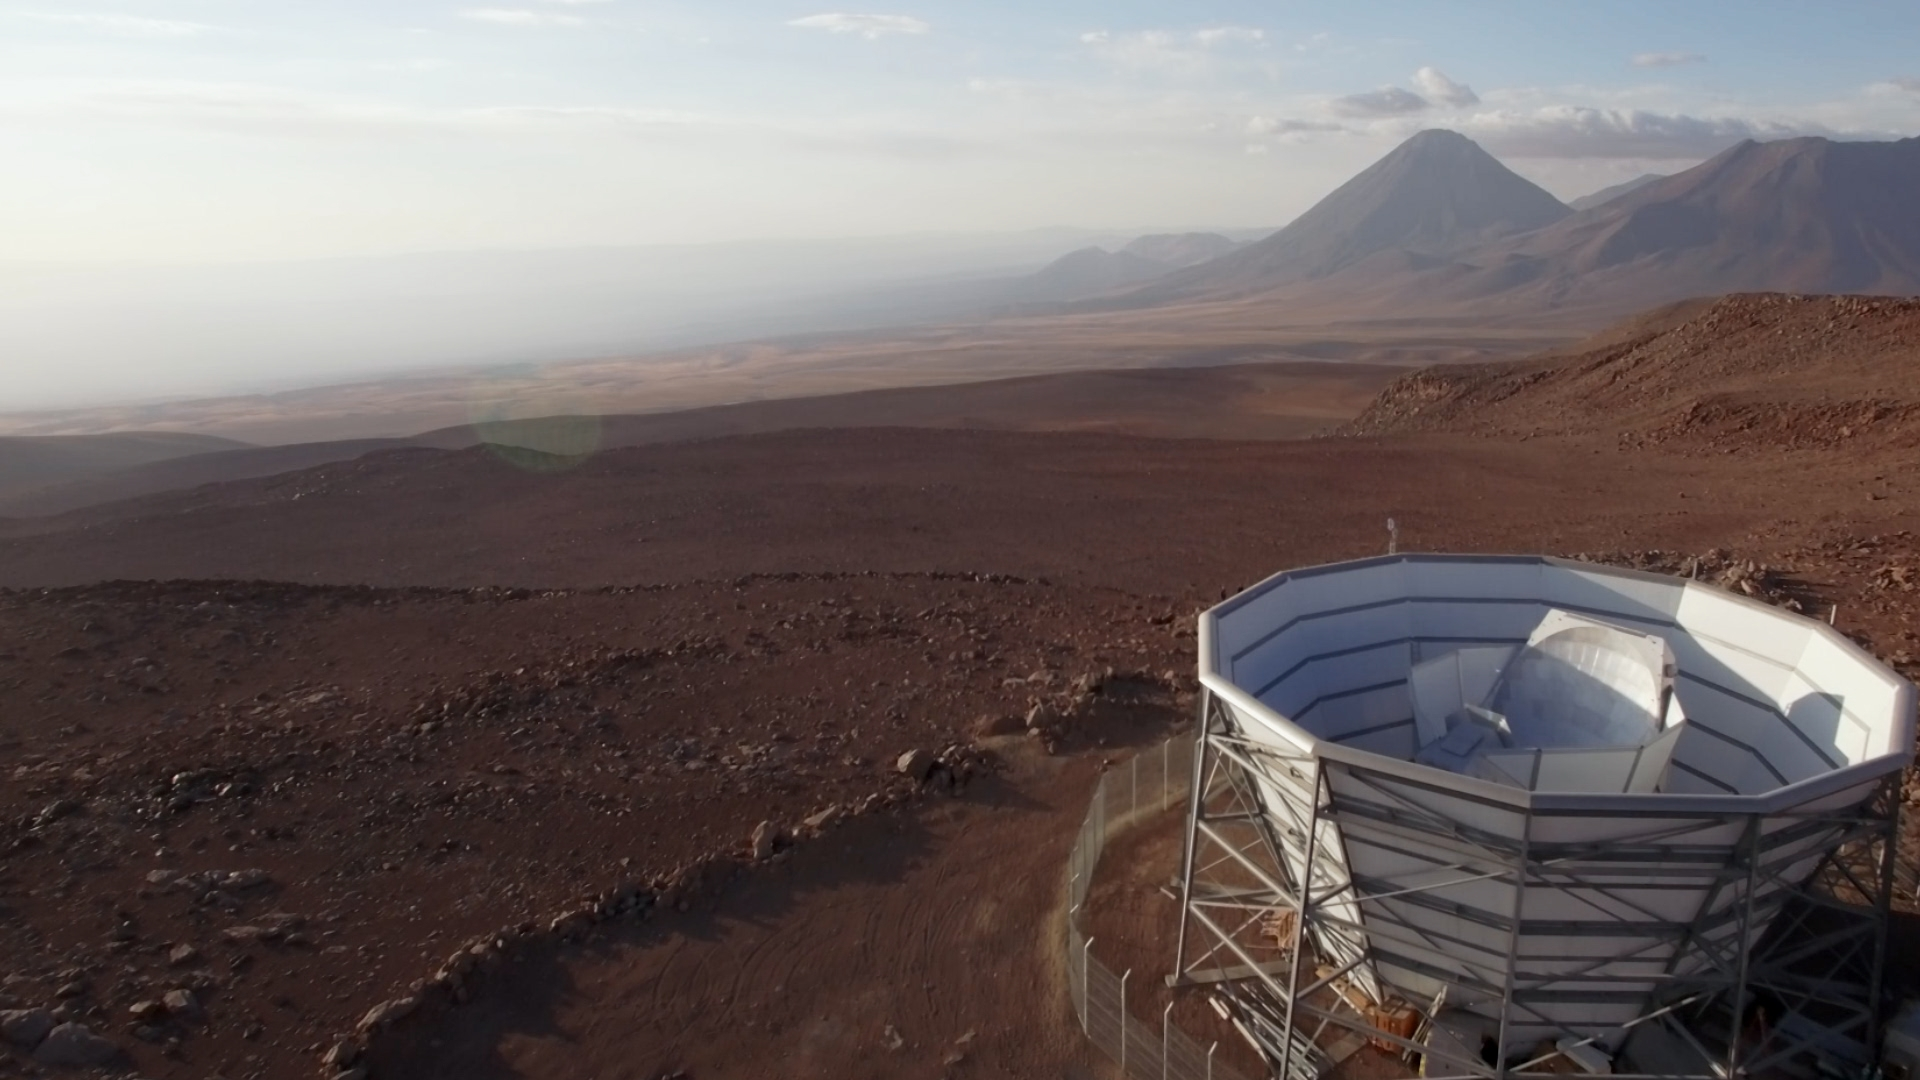
\includegraphics[height=0.15183\textwidth]{figures/telescopes/SO}%
        \vspace{-1pt}

        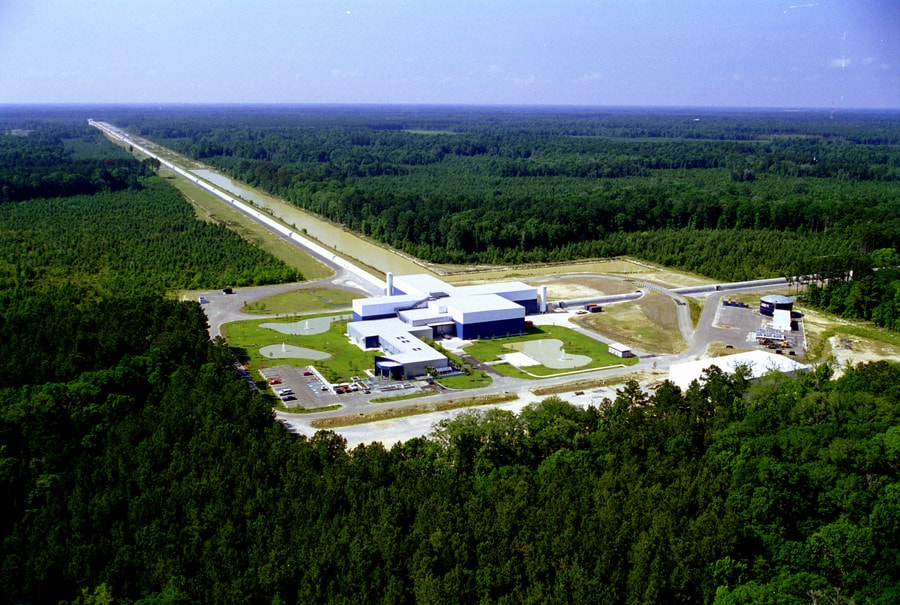
\includegraphics[height=0.18428\textwidth]{figures/telescopes/ligo}%
        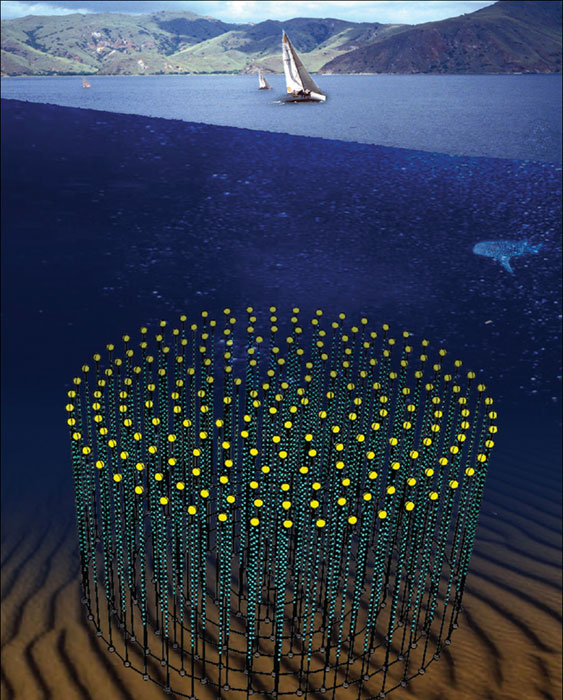
\includegraphics[height=0.18428\textwidth]{figures/telescopes/km3n}%
        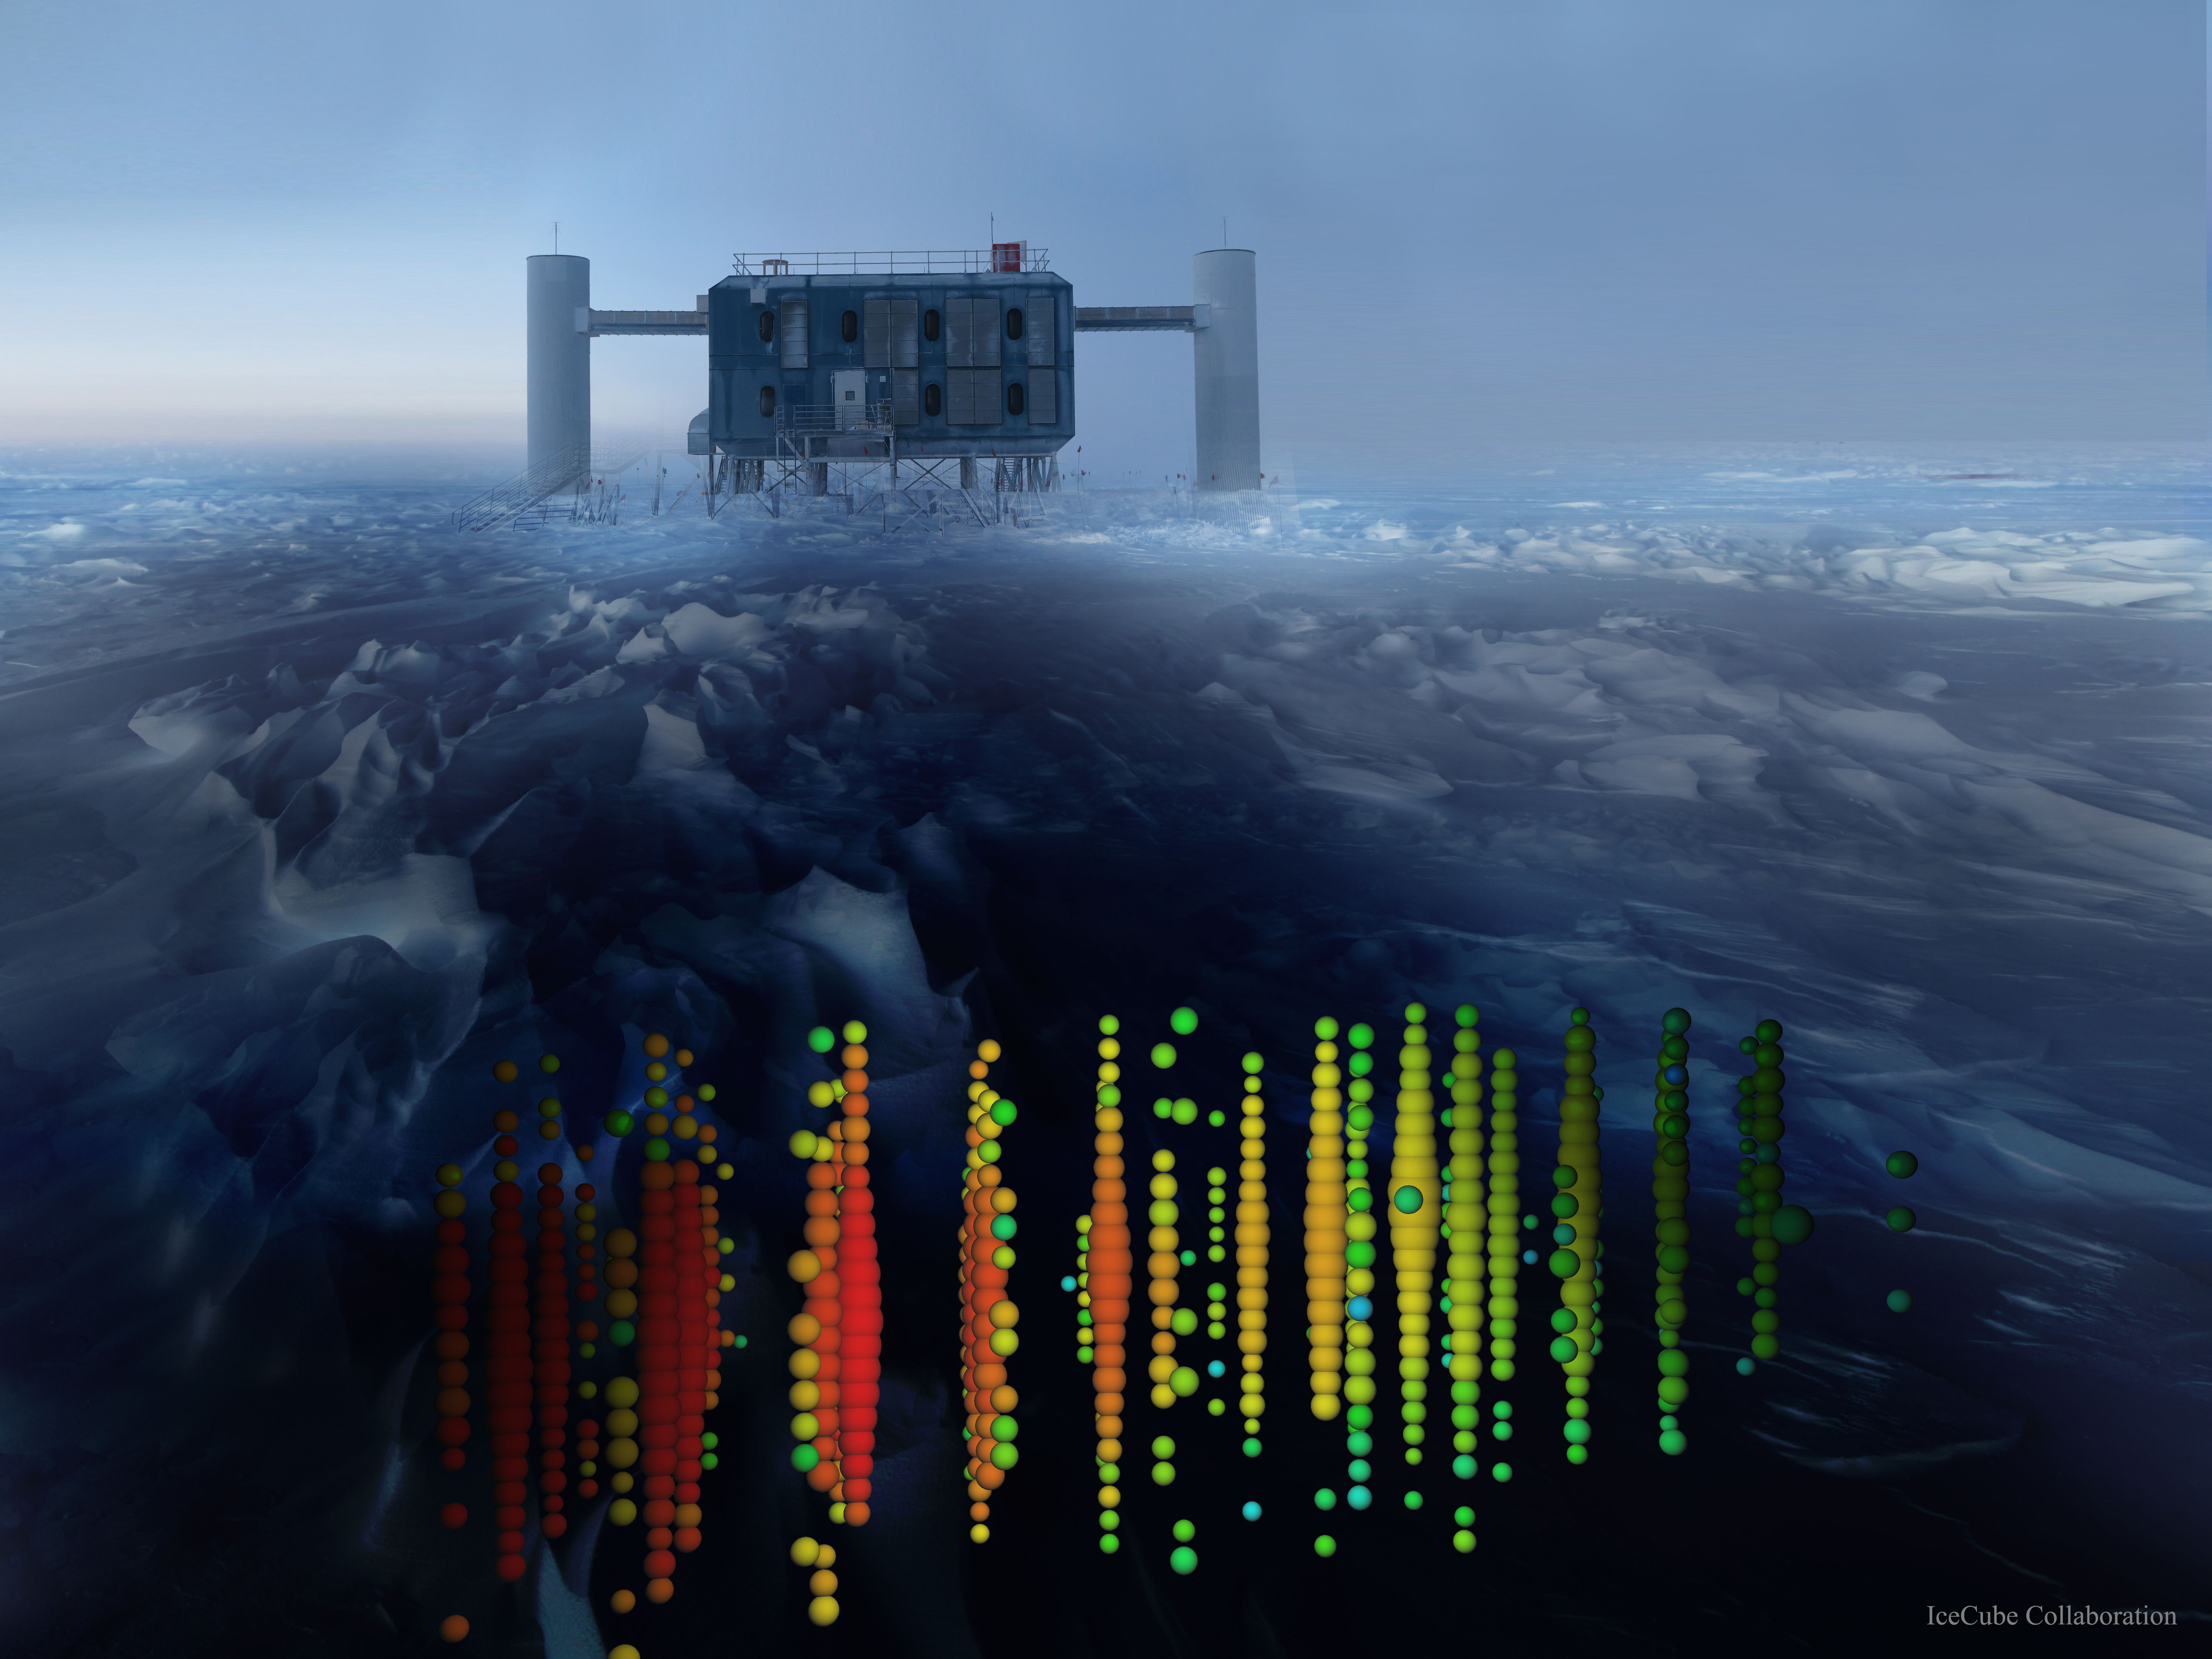
\includegraphics[height=0.18428\textwidth]{figures/telescopes/icecube}%
        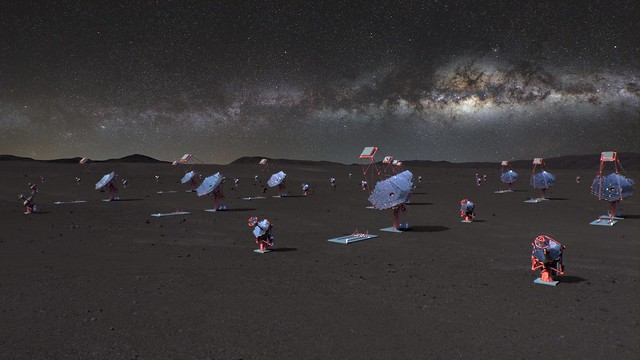
\includegraphics[height=0.18428\textwidth]{figures/telescopes/CTA}%

        \begin{itemize}
            \item We are moving from an age of \textbf{precision} cosmology to \textbf{accurate} cosmology.
            \item \textbf{Systematics} $\gtrsim$ \textbf{statistics}.
            \item Tools risk lagging behind hardware
        \end{itemize}

    \end{columns}
\end{frame}

\begin{frame}
    \frametitle{Tensions in cosmology}
    \begin{columns}
        \column{0.31\textwidth}
        \begin{block}{Hubble tension}
            <+Content+>
        \end{block}
        \column{0.31\textwidth}
        \begin{block}{Weak lensing tension}
            <+Content+>
        \end{block}
        \column{0.31\textwidth}
        \begin{block}{$w_0$/$\Omega_K$/$\nu$}
            <+Content+>
        \end{block}
    \end{columns}
\end{frame}

\begin{frame}
    \frametitle{The real tension in the room}

    \begin{columns}
        \column{0.31\textwidth}
        \begin{block}{Dark tension}
            <+Content+>
        \end{block}
        \column{0.31\textwidth}
        \begin{block}{Initial conditions}
            <+Content+>
        \end{block}
        \column{0.31\textwidth}
        \begin{block}{Quantum gravity}
            <+Content+>
        \end{block}
    \end{columns}

    %importance that even if LCDM is right, and all the previously named tensions/job creators are resolved, we still have a problem
\end{frame}

\begin{frame}
    \frametitle{GAMBIT}
    \framesubtitle{Interdisciplinary case studies}
    %TODO
    what is gambit slide

    KICC event outcomes
\end{frame}

\begin{frame}
    \frametitle{GAMBIT: sub-GeV Dark matter constraints}
    \framesubtitle{Interdisciplinary case studies}
    \student{gambit}{Felix Kahlhoefer et al}{GAMBIT cosmo/DM working group}
    \begin{columns}
        \column{0.56\textwidth}
        \begin{itemize}
            \item Physical model of sub-GeV thermal dark matter with a dark photon mediator~$A$:
        \end{itemize}
        \vspace{-10pt}
        \begin{align*}
        \small
            \mathcal{L}_\text{int} =& -\frac{1}{2} m_{A'}^2 A'^\mu A'_\mu - \frac{1}{4} A'^{\mu\nu}A'_{\mu\nu} -\kappa e A'^\mu \sum_{f} q_f \overline{f} \gamma_\mu f \,,
            \normalsize
        \end{align*}
        \vspace{-15pt}
        \begin{itemize}
            \item Constrain using cosmological, astrophysical, accelerator \& direct detection data.
            \item Bayesian Model comparison of Fermion~$\psi$ vs scalar~$\Phi$ models (scalar preferred).
        \end{itemize}
        \vspace{-10pt}
        \begin{align*}
            \small
            \mathcal{L}_\psi  =& \bar{\psi}(i \slashed{\partial} - m_\text{DM}) \psi + g_\text{DM} A'^\mu \bar{\psi} \gamma_\mu \psi \,,\\
            \mathcal{L}_\Phi  =& |\partial_\mu \Phi|^2 - m_\text{DM}^2 |\Phi|^2 - g_\text{DM}^2 A'_\mu A'^\mu |\Phi|^2 \\ &+ i g_\text{DM} A'^\mu \left[\Phi^\ast (\partial_\mu \Phi) - (\partial_\mu \Phi^\ast) \Phi\right]\,,
        \normalsize
        \end{align*}
        \column{0.44\textwidth}
        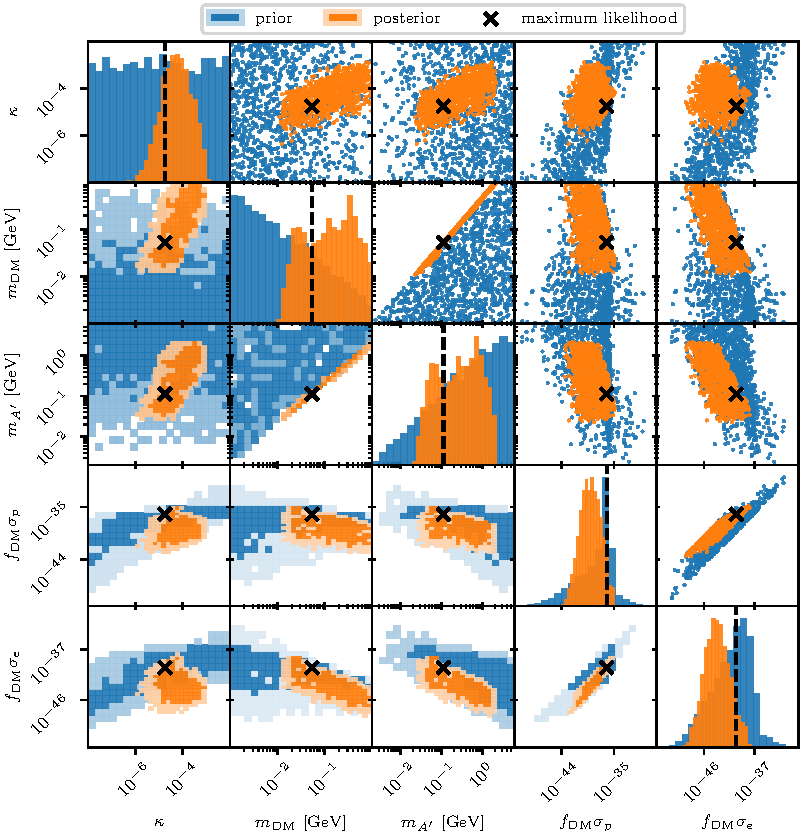
\includegraphics[width=\textwidth]{figures/Bayes_SubGeVDM_fermion_RDprior_allDM_asym_observables.pdf}
    \end{columns}
\end{frame}

\begin{frame}
    \frametitle{Instrumentation + Machine learning: REACH radiometry}
    \only<1>{\student{ian_roque}{Ian Roque}{PhD}}
    \only<2>{\student{sam_leeney}{Sam Leeney}{PhD}}
    \framesubtitle{Interdisciplinary case studies}

\end{frame}

\begin{frame}
    \frametitle{Quantitative Finance$\to$21cm cosmology: \texttt{maxsmooth}}
    \student{harry_bevins}{Harry Bevins}{PhD$\to$KICC fellow}
    \framesubtitle{Interdisciplinary case studies}
\end{frame}

\begin{frame}
    \frametitle{DSTL: }
    \framesubtitle{Interdisciplinary case studies}
    Bayesian OODA loops
\end{frame}


\begin{frame}
    \frametitle{}
    \framesubtitle{Interdisciplinary case studies}
\end{frame}

\begin{frame}
    \frametitle{}
    \framesubtitle{Interdisciplinary case studies}
\end{frame}

\begin{frame}
    \frametitle{unimpeded: PLA for the next generation}
    \student{dily_ong}{Dily Ong}{PhD}
    \begin{columns}
        \column{0.5\textwidth}
        \begin{itemize}
            \item DiRAC 2020 RAC allocation of 30MCPUh
            \item Main goal: Planck Legacy Archive equivalent
            \item Parameter estimation $\to$ Model comparison
            \item MCMC $\to$ Nested sampling
            \item Planck $\to$ $\{\text{Planck}, \text{DESY1}, \text{BAO}, \ldots \}$
            \item Pairwise combinations
            \item Suite of tools for processing these 
                \begin{itemize}
                    \item \texttt{anesthetic} $2.0$
                    \item \texttt{unimpeded} $1.0$
                    \item \texttt{zenodo} archive
                    \item \texttt{margarine}
                \end{itemize}
            \item MCMC chains also available.
            \item Library of bijectors emulators for fast re-use
        \end{itemize}
        \column{0.5\textwidth}
        
\includegraphics[width=\textwidth]{logos/dirac}
        \includegraphics[width=0.5\textwidth,page=21]{figures/himmelblau}%
        \includegraphics[width=0.5\textwidth,page=15]{figures/himmelblau}
    \end{columns}
\end{frame}



\begin{frame}
    \frametitle{Other frontiers}
    Copilot

    ChatGPT

    LLMs/translation between disciplines
    
\end{frame}


\begin{frame}
    \frametitle{Conclusions}
    \framesubtitle{\href{https://www.github.com/handley-lab}{github.com/handley-lab}}
    %TODO
    Images of DiRAC, ERC, URF and PCLtd for resources at my disposal
    \tikz[overlay,remember picture]
        \node[anchor=north east] (A) at ($(current page.north east)+(0,0)$) {
            
\includegraphics[width=0.09\textheight]{figures/students/adam_ormondroyd.jpg}%
            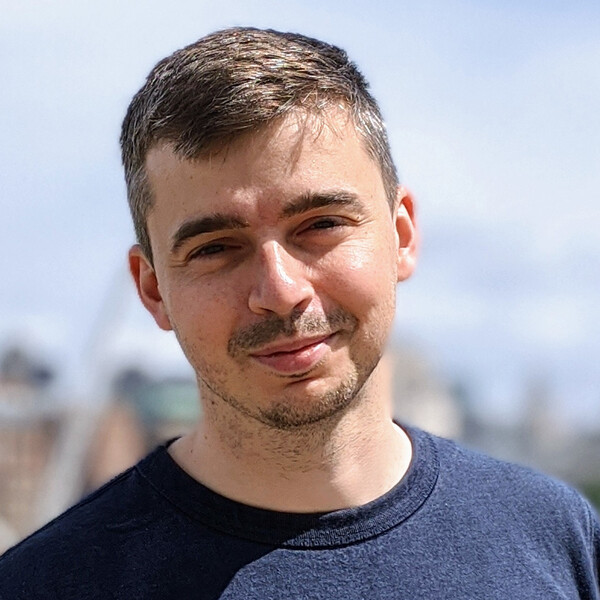
\includegraphics[width=0.09\textheight]{figures/students/david_yallup.jpg}%
            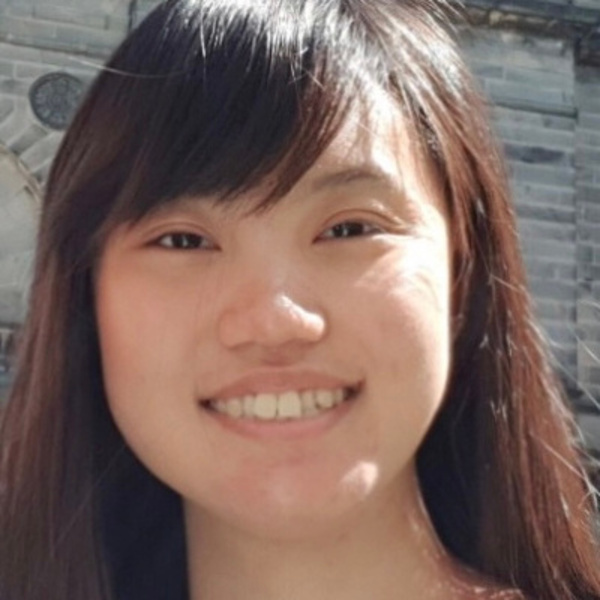
\includegraphics[width=0.09\textheight]{figures/students/dily_ong.jpg}%
            
\includegraphics[width=0.09\textheight]{figures/students/felicity_ibrahim.jpg}%
            
\includegraphics[width=0.09\textheight]{figures/students/george_carter.jpg}%
            
\includegraphics[width=0.09\textheight]{figures/students/harry_bevins.jpg}%
            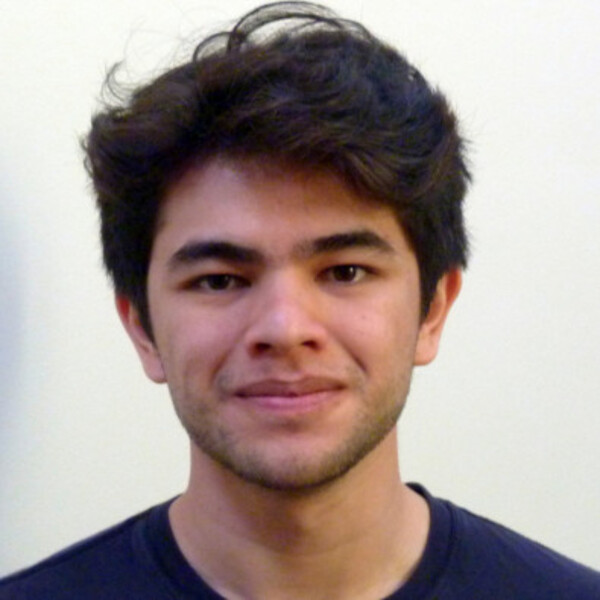
\includegraphics[width=0.09\textheight]{figures/students/ian_roque.jpg}%
            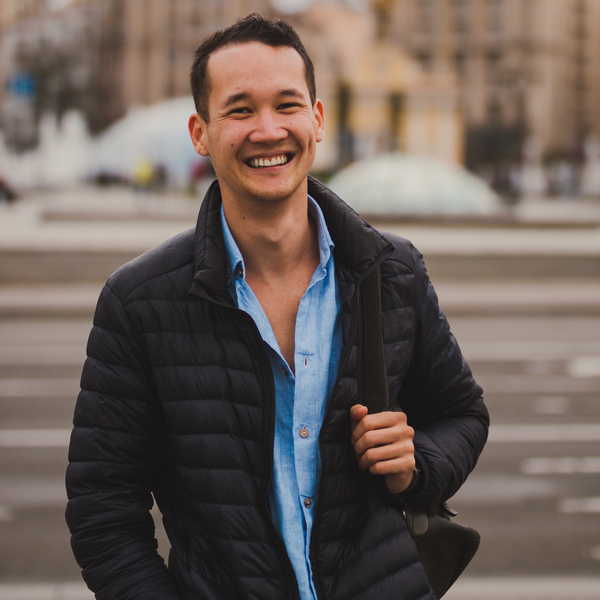
\includegraphics[width=0.09\textheight]{figures/students/kilian_scheutwinkel.jpg}%
            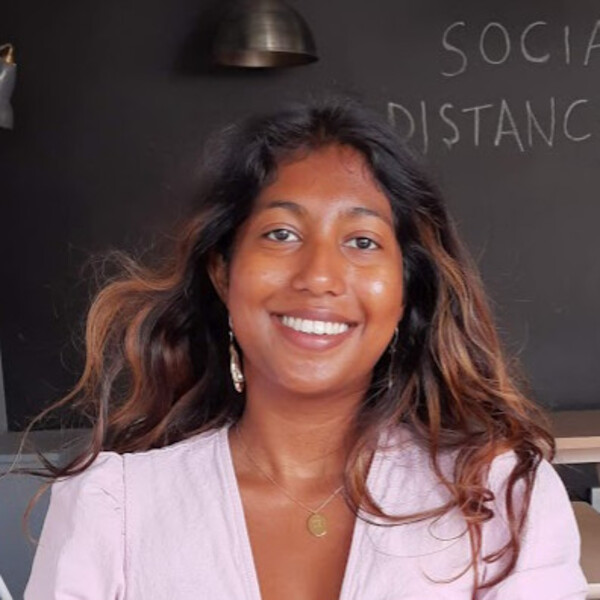
\includegraphics[width=0.09\textheight]{figures/students/metha_prathaban.jpg}%
            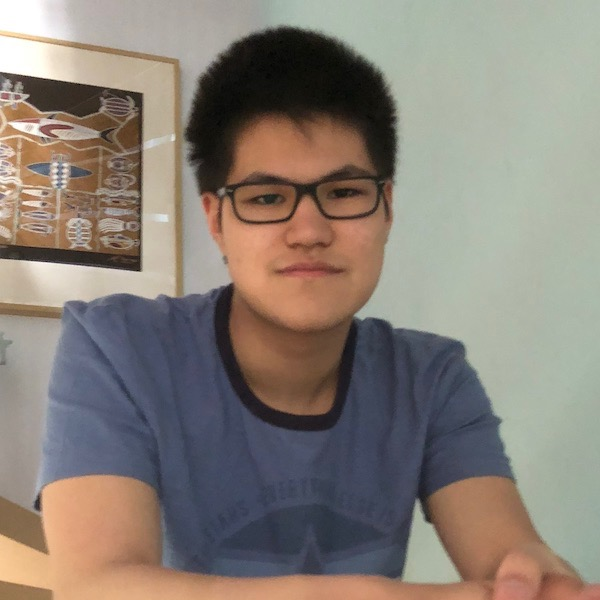
\includegraphics[width=0.09\textheight]{figures/students/namu_kroupa.jpg}%
            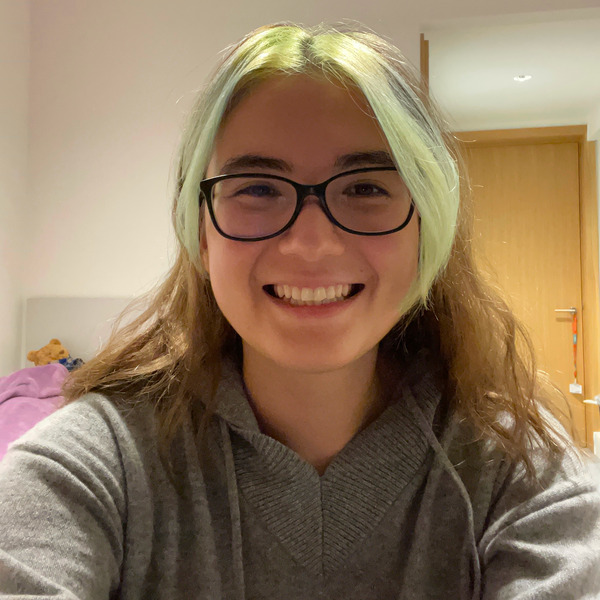
\includegraphics[width=0.09\textheight]{figures/students/sinah_legner.jpg}%
            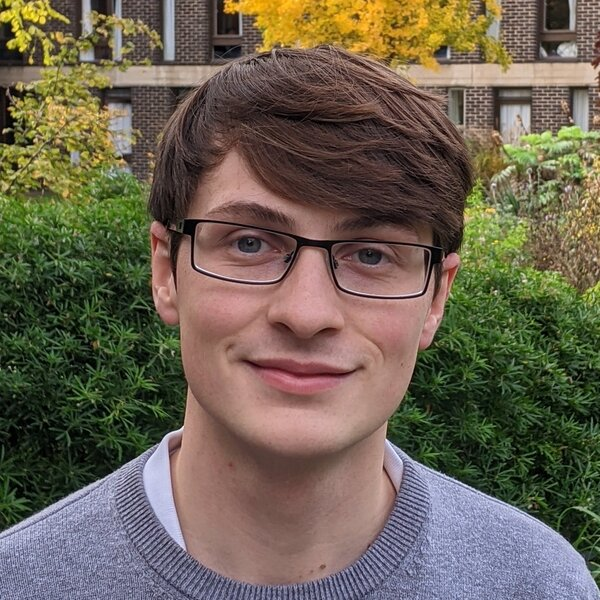
\includegraphics[width=0.09\textheight]{figures/students/thomas_gessey-jones.jpg}%
            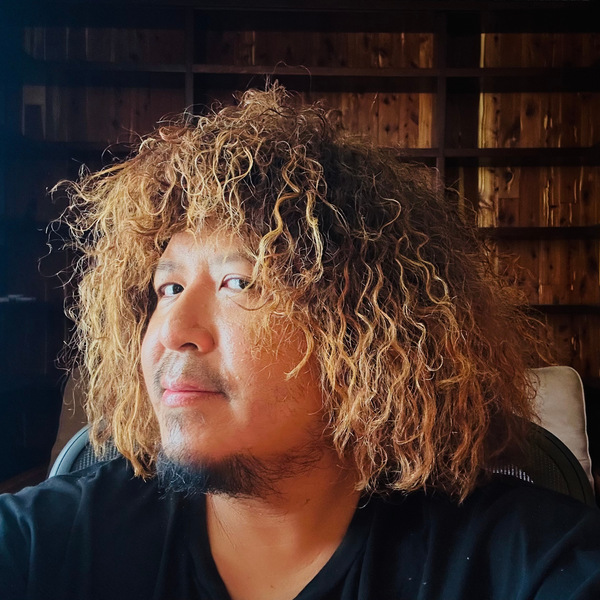
\includegraphics[width=0.09\textheight]{figures/students/tze_goh.jpg}%
            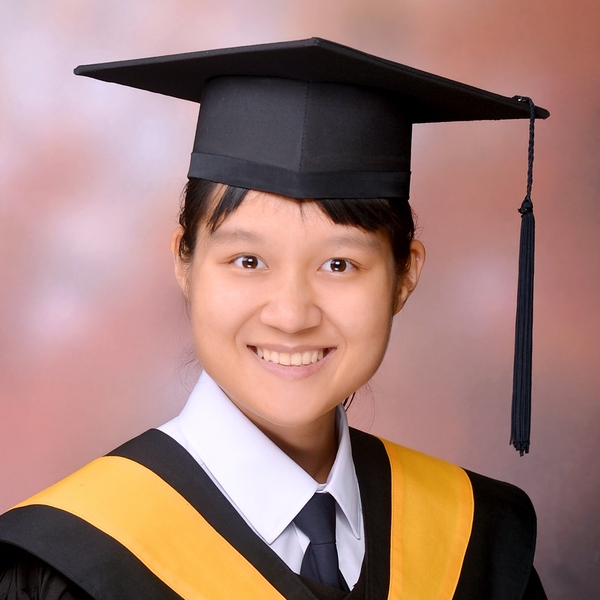
\includegraphics[width=0.09\textheight]{figures/students/wei-ning_deng.jpg}%
    };
\end{frame}

\end{document}
